\documentclass[a4paper,12pt]{article}

\usepackage[utf8]{inputenc}
\usepackage[english,ngerman]{babel}
\selectlanguage{ngerman}

\usepackage[T1]{fontenc}
\usepackage{amsmath}
\usepackage{graphicx}
\usepackage{graphviz}

\usepackage{amsfonts}

\usepackage{url}
\usepackage[colorlinks=false,pdfborder={0 0 0},breaklinks=true]{hyperref}


\begin{document}

\title{Konzeptpapier Lichtsteuerung}
\author{Marius \textbf{Schuller}\\
        Stefan \textbf{Thiemann}\\
		Patrick \textbf{Wildt}}
\maketitle

\tableofcontents

\newpage

\noindent
Hier soll kurz die Grundidee des Schwerpunktprojekts, sowie welche Hardware 
benötigt wird, beschrieben werden.

\section{Einführung}

Im Zuge der Internet-of-Things-Kampagne\footnote{\url{http://www.nextgenerationmedia.de}}
werden immer weitere ``dumme'' Geräte miteinander intelligent vernetzt. Dazu
gehören auch Lichter und Glühbirnen. Zur Vernetzung und Steuerung der Lichter
existieren bereits mehrere aktuelle Technologien. Mit Hilfe einer der
standardisierten Technologie möchten wir einen Controller implementieren,
welcher diese Lichter kontrollieren kann.

\section{Lichtsteuerungs-Technologien}

Üblicherweise möchten Hersteller ein eigenes Produkt-Ökosystem erstellen, aus dem die
Anwender kaum mehr ausbrechen können. In Folge dessen werden eigene Protokolle
implementiert. Beispielsweise bietet \textit{LimitlessLED}
\footnote{\url{http://www.limitlessled.com}} Glühbirnen, welche sich
über 2,4 GHz WLAN in das lokale Netzwerk verbinden können. Für die eigentliche
Steuerung wurde eine eigene API entwickelt. Eine weitere bekannte Technologie ist
\textit{Bluetooth}. Hier ist es derzeit möglich mit Hilfe des \textit{Generic
Attribute Profile}, kurz
\textit{GATT}\footnote{\url{https://de.wikipedia.org/wiki/Bluetooth-Profile}},
ein eigenes Protokoll zu sprechen. Dies wird bei mehreren smarten Glühbirnen
verwendet um ein proprietäres Lichtsteuerungsprotokoll zu implementieren.

\newpage

Die \textit{Bluetooth} Konkurrenten
\textit{Z-Wave}\footnote{\url{http://www.z-wavealliance.org}}, welches sich auf das
so genannte \textit{Home Control}-Szenario konzentriert, sowie
\textit{ZigBee}\footnote{\url{http://www.zigbee.org}},
implementieren jeweils eigene Lichtprotokolle. Diese Protokolle sind jedoch für jeden
Client des Funkstandards nutzbar, sodass die Lichterhersteller kein eigenes Protokoll
implementieren müssen. Der Funkstandard \textit{ZigBee} wird von den namhaften
Herstellern \textit{Philips} und \textit{Osram} verwendet.

Für das Schwerpunktprojekt würden wir uns auf \textit{ZigBee} kompatible Geräte
konzentrieren. Vor allem die Produkte der \textit{Philips hue} Reihe.

\section{Komponenten}

Die eigentliche Logik zur Steuerung der Lichter kann auf einem \textit{RaspberryPi}
implementiert werden. Um den Funkstandard \textit{ZigBee} sprechen zu können wird ein
kompatibles Funkmodul benötigt. Hierfür kann das \textit{RaspBee}-Modul verwendet werden.
Dieses gibt es in zwei Varianten, \textit{Basic} und \textit{Premium}. Während man mit der
Basic-Variante nur mit 5 Knoten sprechen darf, ist dies bei der Premium-Variante
unbegrenzt. Die Lichter würden aus einem \textit{Philips Hue} Starterkit bestehen.

\section{Hardware}

\subsection{RaspBee Premium, Raspberry-Pi Einzeln}

\begin{tabular}{p{2cm}p{4.5cm}p{3cm}p{3cm}}
   Menge & Produkt & Einzelpreis & Gesamtpreis\\
   \hline
   3 & \href{http://www.conrad.de/ce/de/product/1316978/Raspberry-Pi-2-Model-B-1-GB-ohne-Betriebssystem}{RaspberryPi 2} & 42 Euro & 126 Euro\\
   3 & \href{http://www.conrad.de/ce/de/product/1369407/Raspberry-Pi-Erweiterungs-Platine-Zigbee-200-Knotenpunkte-Raspberry-Pi}{RaspBee Premium} & 60 Euro & 180 Euro\\
   3 & \href{http://www.conrad.de/ce/de/product/1314141/Philips-Hue-LED-Leuchtmittel-Erweiterung-E27-9-W-RGB}{Philips Hue LED}
        \newline 1 x 9W A60 E27 & 59 Euro & 177 Euro\\
   \hline
   Gesamtpreis & & & \textbf{483 Euro}\\
\end{tabular}

\subsection{RaspBee Premium, Raspberry-Pi Bundle}

\begin{tabular}{p{2cm}p{4.5cm}p{3cm}p{3cm}}
   Menge & Produkt & Einzelpreis & Gesamtpreis\\
   \hline
   3 & \href{http://www.reichelt.de/Einplatinen-Computer/RASP-2-B-ALL-IN/3/index.html?ACTION=3&GROUPID=6666&ARTICLE=152855}{RaspberryPi 2 Bundle} & 70 Euro & 210 Euro\\
   3 & \href{http://www.conrad.de/ce/de/product/1369407/Raspberry-Pi-Erweiterungs-Platine-Zigbee-200-Knotenpunkte-Raspberry-Pi}{RaspBee Premium} & 60 Euro & 180 Euro\\
   3 & \href{http://www.conrad.de/ce/de/product/1314141/Philips-Hue-LED-Leuchtmittel-Erweiterung-E27-9-W-RGB}{Philips Hue LED}
        \newline 1 x 9W A60 E27 & 59 Euro & 177 Euro\\
   \hline
   Gesamtpreis & & & \textbf{567 Euro}\\
\end{tabular}

\subsection{Hinweis}

Unter Umständen sind Bestandteile der Liste schon im Vorrat der Hochschule oder
der Projektteilnehmer. Je nach Beteiligung der Fachhochschule würden wir für einen
Teil der Kosten aufkommen.

\section{Grobarchitektur}

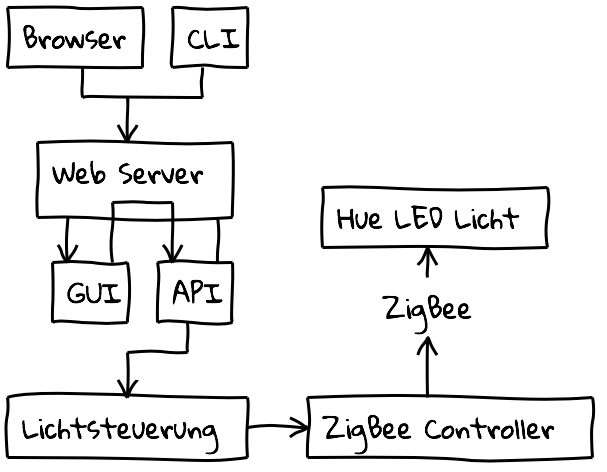
\includegraphics[width=\linewidth]{grobarchitektur}

Die Lichtsteuerung soll aus mehreren miteinander interagierenden Komponenten bestehen, welche in den weiteren Unterkapiteln genauer beschrieben werden.

\subsection{Hue LED Licht}

Die Lampen, welche gesteuert werden sollen, werden in eine herkömmliche Fassung geschraubt. Darüber wird die Lampe mit Strom versorgt. Die Hue LEDs besitzen außerdem einen ZigBee-Chip, mit dem sie Teil eines ZigBee-Netzwerks werden können. In diesem Netzwerk arbeiten sie als \emph{End Device}. Über das ZigBee Light Link Protokoll können die Lampen angesprochen werden und Eigenschaften wie die Farbstärke eingestellt werden.

\subsection{ZigBee Controller}

Der ZigBee Controller ist die eigentliche Funkeinheit. Sie stellt eine rohe Programmierschnittstelle bereit, um auf das ZigBee-Netzwerk zugreifen zu können. Der Controller besteht aus zwei Komponenten. Zum einen dem \emph{RaspBee}, eine aufsteckbare Erweiterungsplatine mit Funkmodul für \emph{Raspberry Pi}, und zum anderen dem \emph{Raspberry Pi} selber. Der \emph{Raspberry Pi}, ein Entwicklungsboard, besitzt eine Reihe an GPIO Pins am Rand des Boards. Das \emph{RaspBee} ist an diese GPIO Pins angepasst und wird dadurch mit Strom gespeist. Weiterhin werden die \emph{UART}-Pins zur seriellen Kommunikation mit einem Treiber, der auf dem \emph{Raspberry Pi} betrieben wird, verwendet.

\subsection{Lichtsteuerung}

Die Lichtsteuerung ist ebenfalls eine Software, die auf dem \emph{Raspberry Pi} betrieben wird. Sie verwendet die Programmierschnittstelle des ZigBee Controllers und stellt eine REST-basierte Webschnittstelle, um die Eigenschaften der Lampen zu kontrollieren.

\subsection{Webserver}

Der Webserver dient primär zur Verteilung des Javascript Codes der \emph{GUI}-Komponente. Weiterhin leitet es Anfragen an die REST-API an die Lichtsteuerung weiter.

\subsection{GUI}

\subsection{CLI}

\end{document}